\documentclass[tikz,border=2pt]{standalone}
\usepackage{amsmath,amssymb}
\usepackage{tikz}
\usetikzlibrary{arrows.meta}

\begin{document}
% A linear program in two variables: linear constraints cut out a polygon, the objective is a
% family of parallel lines, and the best line that still touches the polygon does so at a corner.
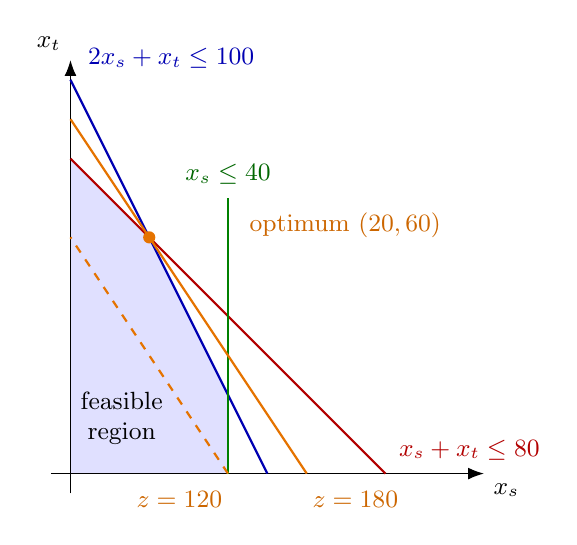
\begin{tikzpicture}[x=0.05cm, y=0.05cm, every node/.style={font=\small}, >={Latex[length=2mm]}]
	\fill[blue!12] (0,0) -- (40,0) -- (40,20) -- (20,60) -- (0,80) -- cycle;
	\draw[->] (-5,0) -- (105,0) node[below right] {$x_s$};
	\draw[->] (0,-5) -- (0,105) node[above left] {$x_t$};
	\draw[blue!70!black, thick] (50,0) -- (0,100);
	\draw[red!70!black, thick] (80,0) -- (0,80);
	\draw[green!50!black, thick] (40,0) -- (40,70);
	\node[blue!70!black, font=\small, anchor=south west] at (2,100.5) {$2x_s+x_t\le100$};
	\node[red!70!black, font=\small, anchor=south west] at (81,1) {$x_s+x_t\le80$};
	\node[green!40!black, font=\small, anchor=south] at (40,71) {$x_s\le40$};
	\draw[orange!90!black, thick, dashed] (40,0) -- (0,60);
	\draw[orange!90!black, thick] (60,0) -- (0,90);
	\node[orange!80!black, anchor=north east] at (41,-2) {$z=120$};
	\node[orange!80!black, anchor=north west] at (59,-2) {$z=180$};
	\fill[orange!90!black] (20,60) circle (2.2pt);
	\node[orange!80!black, font=\small, anchor=west] at (43,63) {optimum $(20,60)$};
	\node[font=\small, align=center] at (13,14) {feasible\\ region};
	\end{tikzpicture}
\end{document}
